\chapter{Sorting and Searching}\label{ch:examples}\label{ch:sorting}\label{ch:searching}

\begin{schemeregion}

\chapquoter{If you keep proving stuff that others have done, getting confidence, increasing the complexities of your solutions---for the fun of it---then one day you'll turn around and discover that nobody actually did that one!\\
And that's the way to become a computer scientist.}{Richard Feynman, \emph{Lectures on Computation}}

This chapter presents two extended examples that use the programming techniques from Chapters~\ref{ch:language}--\ref{ch:data} and analysis ideas from Chapters~\ref{ch:machines}--\ref{ch:cost} to solve some interesting and important problems: sorting and searching.  These examples involve some quite challenging problems and incorporate many of the ideas we have seen up to this point in the book.  Once you understand them, you are well on your way to thinking like a computer scientist!

\LATER{In the final subsection, we return to the question of the growth of computing power introduced in Chapter~\ref{ch:intro} (Section~\ref{sec:growthofcomputing}).  With our increased understanding of how computing work scales with problem size, we can observe and predict how the scale of problems that can be solved by computers changes over time.}

\section{Sorting}\index{general}{sorting|(}

The sorting problem takes two inputs: a list of elements and a comparison procedure.  It outputs a list containing same elements as the input list ordered according to the comparison procedure.  For example, if we sort a list of numbers using \scheme|<| as the comparison procedure, the output is the list of numbers sorted in order from least to greatest.  

Sorting is one of the most widely studied problems in computing, and many different sorting algorithms have been proposed.\cut{\footnote{Donald Knuth's \emph{The Art of Computer Programming} devotes an entire 780-page volume to the problem of sorting and searching.}}\cut{  In this section, we explore a few sorting procedures. } Try to develop a sorting procedure yourself before continuing further.  It may be illuminating to try sorting some items by hand an think carefully about how you do it and how much work it is.  For example, take a shuffled deck of cards and arrange them in sorted order by ranks.  Or, try arranging all the students in your class in order by birthday.  Next, we present and analyze three different sorting procedures.

\subsection{Best-First Sort}\index{general}{best-first-sort}\label{sec:best-first-sort}

A simple sorting strategy is to find the \emph{best} element in the list and put that at the front.  The best element is an element for which the comparison procedure evaluates to \true\ when applied to that element and every other element.  For example, if the comparison function is \scheme|<|, the best element is the lowest number in the list.  This element belongs at the front of the output list.  

The notion of the best element in the list for a given comparison function only makes sense if the comparison function is \definition{transitive}.  This means it has the property that for any inputs \var{a}, \var{b}, and \var{c}, if \scheme|(cf a b)| and \scheme|(cf b c)| are both \schemeresult|true|, the result of \scheme|(cf a c)| must be \schemeresult|true|.  The $<$ function is transitive: $a<b$ and $b<c$ implies $a<c$ for all numbers $a$, $b$, and $c$.  If the comparison function does not have this property, there may be no way to arrange the elements in a single sorted list.  All of our sorting procedures require that the procedure passed as the comparison function is transitive.

Once we can find the best element in a given list, we can sort the whole list by repeatedly finding the best element of the remaining elements until no more elements remain.  To define our best-first sorting procedure, we first define a procedure for finding the best element in the list, and then define a procedure for removing an element from a list.

\shortsection{Finding the Best} The best element in the list is either the first element, or the best element from the rest of the list.  Hence, we define \scheme|list-find-best| recursively.  An empty list has no best element, so the base case is for a list that has one element.  When the input list has only one element, that element is the best element.  If the list has more than one element, the best element is the better of the first element in the list and the best element of the rest of the list.

To pick the better element from two elements, we define the \scheme|pick-better| procedure that takes three inputs: a comparison function and two values.  
\begin{schemedisplay}
(define (pick-better cf p1 p2) (if (cf p1 p2) p1 p2))
\end{schemedisplay}

Assuming the procedure passed as \scheme|cf| has constant running time, the running time of \scheme|pick-better| is constant.  For most of our examples, we use the \scheme|<| procedure as the comparison function.  For arbitrary inputs, the running time of \scheme|<| is not constant since in the worst case performing the comparison requires examining every digit in the input numbers.  But, if the maximum value of a number in the input list is limited, then we can consider \scheme|<| a constant time procedure since all of the inputs passed to it are below some fixed size.

We use \scheme|pick-better| to define \scheme|list-find-best|:
\begin{schemedisplay}
(define (list-find-best cf p)
  (if (null? (cdr p)) (car p)
      (pick-better cf (car p) (list-find-best cf (cdr p)))))
\end{schemedisplay}

We use $n$ to represent the number of elements in the input list \scheme|p|.  An application of \scheme|list-find-best| involves $n-1$ recursive applications since each one passes in \scheme|(cdr p)| as the new \scheme|p| operand and the base case stops when the list has one element left.  The running time for each application (excluding the recursive application) is constant since it involves only applications of the constant time procedures \scheme|null?|, \scheme|cdr|, and \scheme|pick-better|.  So, the total running time for \scheme|list-find-best| is in $\Theta(n)$; it scales linearly with the length of the input list.

\shortsection{Deleting an Element}  To implement best first sorting, we need to produce a list that contains all the elements of the original list except for the best element, which will be placed at the front of the output list.  We define a procedure, \scheme|list-delete|, that takes as inputs a List and a Value, and produces a List that contains all the elements of the input list in the original order except for the first element that is equal to the input value.
\begin{schemedisplay}
(define (list-delete p el)
  (if (null? p) null
      (if (equal? (car p) el) (cdr p) ; found match, skip this element
          (cons (car p) (list-delete (cdr p) el)))))
\end{schemedisplay}

\index{general}{equal?}We use the \scheme|equal?| procedure to check if the element matches instead of \scheme|=| so the \scheme|list-delete| procedure works on elements that are not just  Numbers.  The \scheme|equal?| procedure behaves identically to \scheme|=| when both inputs are Numbers, but also works sensibly on many other datatypes including Booleans, Characters, Pairs, Lists, and Strings.  Since we assume the sizes of the inputs to \scheme|equal?| are bounded, we can consider \scheme|equal?| to be a constant time procedure (even though it would not be constant time on arbitrary inputs).

The worst case running time for \scheme|list-delete| occurs when no element in the list matches the value of \scheme|el| (in the best case, the first element matches and the running time does not depend on the length of the input list at all).  We use $n$ to represent the number of elements in the input list.  There can be up to $n$ recursive applications of \scheme|list-delete|.  Each application has constant running time since all of the procedures applied (except the recursive call) have constant running times.  Hence, the total running time for \scheme|list-delete| is in $\Theta(n)$ where $n$ is the length of the input list.

\shortsection{Best-First Sorting}  We define \scheme|list-sort-best-first| using \scheme|list-find-best| and \scheme|list-delete|:
\begin{schemedisplay}
(define (list-sort-best-first cf p)
  (if (null? p) null
      (cons (list-find-best cf p) 
            (list-sort-best-first cf (list-delete p (list-find-best cf p))))))
\end{schemedisplay}

The running time of the \scheme|list-sort-best-first| procedure grows quadratically with the length of the input list.  We use $n$ to represent the number of elements in the input list.  There are $n$ recursive applications since each application of \scheme|list-delete| produces an output list that is one element shorter than its input list.  In addition to the constant time procedures (\scheme|null?| and \scheme|cons|), the body of \scheme|list-sort-best-first| involves two applications of \scheme|list-find-best| on the input list, and one application of \scheme|list-delete| on the input list. \sidepicturenocap{1.0}{images/pokersort-iStock_000001481019XSmall.jpg}

Each of these applications has running time in $\Theta(m)$ where $m$ is the length of the input list to \scheme|list-find-best| and \scheme|list-delete| (we use $m$ here to avoid confusion with $n$, the length of the first list passed into \scheme|list-sort-best-first|).  In the first application, this input list will be a list of length $n$, but in later applications it will be involve lists of decreasing length: $n-1$, $n-2$, $\cdots$, 1.  Hence, the \emph{average} length of the input lists to \scheme|list-find-best| and \scheme|list-delete| is approximately $\frac{n}{2}$.  Thus, the average running time for each of these applications is in $\Theta(\frac{n}{2})$, which is equivalent to $\Theta(n)$.  

There are three applications (two of \scheme|list-find-best| and one of \scheme|list-delete|) for each application of \scheme|list-sort-best-first|, so the total running time for each application is in $\Theta(3n)$, which is equivalent to $\Theta(n)$.  

There are $n$ recursive applications, each with average running time in $\Theta(n)$, so the running time for \scheme|list-sort-best-first| is in $\Theta(n^2)$.  This means doubling the length of the input list quadruples the expected running time, so we predict that sorting a list of 2000 elements to take approximately four times as long as sorting a list of 1000 elements.

\shortsection{Let expression} Each application of the \scheme|list-sort-best-first| procedure involves two evaluations of \scheme|(list-find-best cf p)|, a procedure with running time in $\Theta(n)$ where $n$ is the length of the input list.  \index{general}{let expression}

The result of both evaluations is the same, so there is no need to evaluate this expression twice.  We could just evaluate \scheme|(list-find-best cf p)| once and reuse the result.  One way to do this is to introduce a new procedure using a lambda expression and pass in the result of \scheme|(list-find-best cf p)| as a parameter to this procedure so it can be used twice:
\begin{schemedisplay}
(define (list-sort-best-first-nodup cf p)
   (if (null? p) null
       ((lambda (best)
          (cons best (list-sort-best-first-nodup cf (list-delete p best))))
        (list-find-best cf p))))
\end{schemedisplay}

This procedure avoids the duplicate evaluation of \scheme|(list-find-best cf p)|, but is quite awkward to read and understand.  

Scheme provides the let expression special form to avoid this type of duplicate work more elegantly.  The grammar for the let expression is: 

\begin{bnfgrammarm}{LetExpression}
\bnfrule{Expression}{\nonterminal{LetExpression}}
\bnfrule{LetExpression}{\scheme|(let (\Bindings) \Expression)|}
\bnfrule{Bindings}{\nonterminal{Binding} \nonterminal{Bindings}}
\bnfrule{Bindings}{$\epsilon$}
\bnfrule{Binding}{\scheme|(\NameG \ExpressionG)|}
\end{bnfgrammarm}

The evaluation rule for the let expression is:
\begin{quote}
\bold{Evaluation Rule 6: Let expression.}  To evaluate a let expression, evaluate each binding in order. To evaluate each binding, evaluate the binding expression and bind the name to the value of that expression. Then, the value of the let expression is the value of the body expression evaluated with the names in the expression that match binding names substituted with their bound values.
\end{quote}

A let expression can be transformed into an equivalent application expression.  The let expression 
\begin{schemedisplay}
(let ((\Namea \Expressiona) (\Nameb \Expressionb) 
      \cdots (\Namek \Expressionk))
  \ExpressionBody)
\end{schemedisplay}
is equivalent to the application expression: 
\begin{schemedisplay}
((lambda (\Namea \Nameb \ldots \Namek) \ExpressionBody)
 \Expressiona \Expressionb \ldots \Expressionk)
\end{schemedisplay}
 
The advantage of the let expression syntax is it puts the expressions next to the names to which they are bound. Using a let expression, we define \scheme|list-sort-best-first-let| to avoid the duplicate evaluations:
\begin{schemedisplay}
(define (list-sort-best-first-let cf p)
  (if (null? p) null
      (let ((best (list-find-best cf p)))
        (cons best (list-sort-best-first-let cf (list-delete p best))))))
\end{schemedisplay}

This runs faster than \scheme|list-sort-best-first| since it avoids the duplicate evaluations, but the asymptotic asymptotic running time is still in $\Theta(n^2)$: there are $n$ recursive applications of \scheme|list-sort-best-first-let| and each application involves linear time applications of \scheme|list-find-best| and \scheme|list-delete|.  Using the let expression improves the actual running time by avoiding the duplicate work, but does not impact the asymptotic growth rate since the duplicate work is hidden in the constant factor.

\beforeex
\begin{exercise}
What is the best case input for \scheme|list-sort-best-first|?  What is its asymptotic running time on the best case input?
\solution{\LATER{}}
\end{exercise}
\afterex

\beforeex
\begin{exercise} \label{exercise:timingsorts} 
Use the \scheme|time| special form (Section~\ref{sec:measuringcost}) to experimentally measure the evaluation times for the \scheme|list-sort-best-first-let| procedure. Do the results match the expected running times based on the $\Theta(n^2)$ asymptotic running time?  

You may find it helpful to define a procedure that constructs a list containing $n$ random elements.  To generate the random elements use the built-in procedure \scheme|random| that takes one number as input and evaluates to a pseudorandom number between 0 and one less than the value of the input number.  Be careful in your time measurements that you do not include the time required to generate the input list.\index{general}{random}
\solution{\LATER{}}
\end{exercise}
\afterex

%\ex{Compare the running times of the original \scheme|list-sort-best-first| procedure and the \scheme|list-sort-best-first-let| procedure that avoids duplicate work.  Are the timing results consistent with the analysis?} 

\beforeex
\begin{exercise} \greenstar 
Define the \scheme|list-find-best| procedure using the \scheme|list-accumulate| procedure from Section~\ref{sec:generic} and evaluate its asymptotic running time.
\solution{\LATER{}}
\end{exercise}
\afterex


\beforeex
\begin{exercise} \goldstar 
Define and analyze a \scheme|list-sort-worst-last| procedure that sorts by finding the worst element first and putting it at the end of the list.
\solution{\LATER{}}
\end{exercise}
\afterex

\subsection{Insertion Sort}

The \scheme|list-sort-best-first| procedure seems quite inefficient.  For every output element, we are searching the whole remaining list to find the best element, but do nothing of value with all the comparisons that were done to find the best element.  

An alternate approach is to build up a sorted list as we go through the elements. Insertion sort works by putting the first element in the list in the right place in the list that results from sorting the rest of the elements.  

First, we define the \scheme|list-insert-one| procedure that takes three inputs: a comparison procedure, an element, and a List.  The input List must be sorted according to the comparison function.  As output, \scheme|list-insert-one| produces a List consisting of the elements of the input List, with the input element inserts in the right place according to the comparison function.

\begin{schemedisplay}
(define (list-insert-one cf el p) ; requires: p is sorted by cf
  (if (null? p) (list el)
      (if (cf el (car p)) (cons el p)
          (cons (car p) (list-insert-one cf el (cdr p))))))
\end{schemedisplay}

The running time for \scheme|list-insert-one| is in $\Theta(n)$ where $n$ is the number of elements in the input list.  In the worst case, the input element belongs at the end of the list and it makes $n$ recursive applications of \scheme|list-insert-one|.  Each application involves constant work so the overall running time of \scheme|list-insert-one| is in $\Theta(n)$.

To sort the whole list, we insert each element into the list that results from sorting the rest of the elements:

\begin{schemedisplay}
(define (list-sort-insert cf p)
  (if (null? p) null
      (list-insert-one cf (car p) (list-sort-insert cf (cdr p)))))
\end{schemedisplay}

\sidepicturenocap{0.22}{images/insertion-iStock_000004216447XSmall.jpg}
Evaluating an application of \scheme|list-sort-insert| on a list of length $n$ involves $n$ recursive applications.  The lengths of the input lists in the recursive applications are $n-1$, $n-2$, $\ldots$, 0.  Each application involves an application of \scheme|list-insert-one| which has linear running time.  The average length of the input list over all the applications is approximately $\frac{n}{2}$, so the average running time of the \scheme|list-insert-one| applications is in $\Theta(n)$.  There are $n$ applications of \scheme|list-insert-one|, so the total running time is in $\Theta(n^2)$.  

\beforeex
\begin{exercise}
We analyzed the worst case running time of \scheme|list-sort-insert| above.  Analyze the best case running time.  Your analysis should identify the inputs for which \scheme|list-sort-insert| runs fastest, and describe the asymptotic running time for the best case input.
\solution{\LATER{}}
\end{exercise}
\afterex

\beforeex
\begin{exercise}
Both the \scheme|list-sort-best-first-sort| and \scheme|list-sort-insert| procedures have asymptotic running times in $\Theta(n^2)$.  This tells us how their worst case running times grow with the size of the input, but isn't enough to know which procedure is faster for a particular input.  For the questions below, use both analytical and empirical analysis to provide a convincing answer.
\begin{subexerciselist}
\item How do the actual running times of \scheme|list-sort-best-first-sort| and \scheme|list-sort-insert| on typical inputs compare?  
\solution{\LATER{}}
\item Are there any inputs for which \scheme|list-sort-best-first| is faster than \scheme|list-sort-insert|?  
\solution{\LATER{}}
\item For sorting a long list of $n$ random elements, how long does each procedure take?  (See Exercise~\ref{exercise:timingsorts} for how to create a list of random elements.)
\solution{\LATER{}}
\end{subexerciselist}
\end{exercise}
\afterex


\subsection{Quicker Sorting}

Although insertion sort is typically faster than best-first sort, its running time is still scales quadratically with the length of the list.  If it takes 100 milliseconds (one tenth of a second) to sort a list containing 1000 elements using \scheme|list-sort-insert|\cut{ (on my laptop, it takes about 120 milliseconds to sort a random list of 1000 elements)}, we expect it will take four ($=2^2$) times as long to sort a list containing 2000 elements, and a million times ($=1000^2$) as long (over a day!) to sort a list containing one million ($1000*1000$) elements. Yet computers routinely need to sort lists containing many millions of elements (for example, consider processing credit card transactions or analyzing the data collected by a super collider).

The problem with our insertion sort is that it divides the work unevenly into inserting one element and sorting the rest of the list.  This is a very unequal division.  Any sorting procedure that works by considering one element at a time and putting it in the sorted position as is done by \scheme|list-sort-find-best| and \scheme|list-sort-insert| has a running time in $\Omega(n^2)$.  We cannot do better than this with this strategy since there are $n$ elements, and the time required to figure out where each element goes is in $\Omega(n)$.  

To do better, we need to either reduce the number of recursive applications needed (this would mean each recursive call results in more than one element being sorted), or reduce the time required for each application.  The approach we take is to use each recursive application to divide the list into two approximately equal-sized parts, but to do the division in such a way that the results of sorting the two parts can be combined directly to form the result.  We partition the elements in the list so that all elements in the first part are less than (according to the comparison function) all elements in the second part.  \LATER{This is similar to how we performed fast exponentiation in Example~\ref{example:exponentiation}.  In that instance, we reduced the number of multiplication operations needed from being in $\Theta(n)$ to in $\Theta(\log_2 n)$ by dividing the work into two equal-sized parts.  For list sorting, we will see that dividing the problem into two problems of approximately equal size has similar benefits.}

Our first attempt is to modify \scheme|insert-one| to partition the list into two parts.  This approach does not produce a better-than-quadratic time sorting procedure because of the inefficiency of accessing list elements; however, it leads to insights for producing a quicker sorting procedure.

First, we define a \scheme|list-extract| procedure that takes as inputs a list and two numbers indicating the start and end positions, and outputs a list containing the elements of the input list between the start and end positions:
\begin{schemedisplay}
(define (list-extract p start end)
  (if (= start 0)
      (if (= end 0) null
          (cons (car p) (list-extract (cdr p) start (- end 1))))
      (list-extract (cdr p) (- start 1) (- end 1))))
\end{schemedisplay}

The running time of the \scheme|list-extract| procedure is in $\Theta(n)$ where $n$ is the number of elements in the input list.  The worst case input is when the value of \scheme|end| is the length of the input list, which means there will be $n$ recursive applications, each involving a constant amount of work.  

We use \scheme|list-extract| to define procedures for obtaining first and second halves of a list (when the list has an odd number of elements, we put the middle element in the second half of the list):

\begin{schemedisplay}
(define (list-first-half p)
  (list-extract p 0 (floor (/ (list-length p) 2))))
  
(define (list-second-half p)
  (list-extract p (floor (/ (list-length p) 2)) (list-length p)))
\end{schemedisplay}

The \scheme|list-first-half| and \scheme|list-second-half| procedures use \scheme|list-extract| so their running times are linear in the number of elements in the input list.  

The \scheme|list-insert-one-split| procedure inserts an element in sorted order by first splitting the list in halves and then recursively inserting the new element in the appropriate half of the list:

\begin{schemedisplay}
(define (list-insert-one-split cf el p) ; requires: p is sorted by cf
  (if (null? p) (list el)      
      (if (null? (cdr p))
          (if (cf el (car p)) (cons el p) (list (car p) el))
          (let ((front (list-first-half p)) (back (list-second-half p)))     
            (if (cf el (car back))
                (list-append (list-insert-one-split cf el front) back)
                (list-append front (list-insert-one-split cf el back)))))))
\end{schemedisplay}

In addition to the normal base case when the input list is \schemeresult|null|, we need a special case when the input list has one element.  If the element to be inserted is before this element, the output is produced using \scheme|cons|; otherwise, we produce a list of the first (only) element in the list followed by the inserted element.  

In the recursive case, we use the \scheme|list-first-half| and \scheme|list-second-half| procedures to split the input list and bind the results of the first and second halves to the \scheme|front| and \scheme|back| variables so we do not need to evaluate these expressions more than once.

Since the list passed to \scheme|list-insert-one-split| is required to be sorted, the elements in \scheme|front| are all less than the first element in \scheme|back|.  Hence, only one comparison is needed to determine which of the sublists contains the new element: if the element is before the first element in \scheme|back| it is in the first half, and we produce the result by appending the result of inserting the element in the front half with the back half unchanged; otherwise, it is in the second half, so we produce the result by appending the front half unchanged with the result of inserting the element in the back half.

To analyze the running time of \scheme|list-insert-one-split| we determine the number of recursive calls and the amount of work involved in each application.  We use $n$ to denote the number of elements in the input list.  Unlike the other recursive list procedures we have analyzed, the number of recursive applications of \scheme|list-insert-one-split| does not scale linearly with the length of the input list.  The reason for this is that instead of using \scheme|(cdr p)| in the recursive call, \scheme|list-insert-one-split| passes in either the \scheme|front| or \scheme|back| value which is the result of \scheme|(first-half p)| or \scheme|(second-half p)| respectively.  The length of the list produced by these procedures is approximately $\frac{1}{2}$ the length of the input list.  With each recursive application, the size of the input list is halved.  This means, \emph{doubling} the size of the input list only adds one more recursive application.  This means the number of recursive calls is logarithmic in the size of the input.\index{general}{logarithmic growth}

Recall that the \emph{logarithm} ($\log_b$) of a number $n$ is the number $x$ such that $b^x = n$ where $b$ is the \emph{base} of the logarithm.  In computing, we most commonly encounter logarithms with base 2.  Doubling the input value increases the value of its logarithm base two by one: $\log_{2} 2n = 1 + \log_{2} n$.  Changing the base of a logarithm from $k$ to $b$ changes the value by the constant factor (see Section~\ref{sec:inputsize}), so inside the asymptotic operators a constant base of a logarithm does not matter.  Thus, when the amount of work increases by some constant amount when the input size doubles, we write that the growth rate is in $\Theta(\log n)$ without specifying the base of the logarithm.  %Thus, the number of recursive applications of \scheme|list-insert-one-split| is in $\Theta(\log n)$ since doubling the size of the input requires one more recursive application.  

Each \scheme|list-insert-one-split| application applies \scheme|list-append| to a first parameter that is either the front half of the list or the result of inserting the element in the front half of the list.  In either case, the length of the list is approximately $\frac{n}{2}$.  The running time of \scheme|list-append| is in $\Theta(m)$ where $m$ is the length of the first input list.  So, the time required for each \scheme|list-insert-one-split| application is in $\Theta(n)$ where $n$ is the length of the input list to \scheme|list-insert-one-split|.  

The lengths of the input lists to \scheme|list-insert-one-split| in the recursive calls are approximately $\frac{n}{2}$, $\frac{n}{4}$, $\frac{n}{8}$, $\ldots$, 1, since the length of the list halves with each call.  The summation has $\log_2 n$ terms, and the sum of the list is $n$, so the average length input is $\frac{n}{\log_2 n}$.  Hence, the total running time for the \scheme|list-append| applications in each application of \scheme|list-insert-one-split| is in $\Theta(\log_2 n \times \frac{n}{\log_2 n}) = \Theta(n)$.

The analysis of the applications of \scheme|list-first-half| and \scheme|list-second-half| is similar: each requires running time in $\Theta(m)$ where $m$ is the length of the input list, which averages $\frac{n}{\log_2 n}$ where $n$ is the length of the input list of \scheme|list-insert-one-split|.  Hence, the total running time for \scheme|list-insert-one-split| is in $\Theta(n)$.

The \scheme|list-sort-insert-split| procedure is identical to \scheme|list-sort-insert| (except for calling \scheme|list-insert-one-split|):
\begin{schemedisplay}
(define (list-sort-insert-split cf p)
  (if (null? p) null
      (list-insert-one-split cf (car p) (list-sort-insert-split cf (cdr p)))))
\end{schemedisplay}

Similarly to \scheme|list-sort-insert|, \scheme|list-sort-insert-split| involves $n$ applications of \scheme|list-insert-one-split|, and the average length of the input list is $\frac{n}{2}$.  Since \scheme|list-sort-insert-split| involves $\Theta(n)$ applications of \scheme|list-insert-one-split| with average input list length of $\frac{n}{2}$, the total running time for \scheme|list-sort-insert-split| is in $\Theta(n^2)$.  Because of the cost of evaluating the \scheme|list-append|, \scheme|list-first-half|, and \scheme|list-second-half| applications, the change to splitting the list in halves has not improved the asymptotic performance; in fact, because of all the extra work in each application, the actual running time is higher than it was for \scheme|list-sort-insert|.

The problem with our \scheme|list-insert-one-split| procedure is that the \scheme|list-first-half| and \scheme|list-second-half| procedures have to \scheme|cdr| down the whole list to get to the middle of the list, and the \scheme|list-append| procedure needs to walk through the entire input list to put the new element in the list.  All of these procedures have running times that scale linearly with the length of the input list.  To use the splitting strategy effectively, we need is a way to get to the middle of the list quickly.  With the standard list representation this is impossible: it requires one \scheme|cdr| application to get to the next element in the list, so there is no way to access the middle of the list without using at least $\frac{n}{2}$ applications of \scheme|cdr|.  To do better, we need to change the way we represent our data. The next subsection introduces such a structure; in Section~\ref{sec:quicksort} shows a way of sorting efficiently using lists directly by changing how we split the list.

\subsection{Binary Trees}\label{sec:binary-trees}

The data structure we will use is known as a \definition{sorted binary tree}\index{general}{binary tree}\index{general}{tree}.  While a list provides constant time procedures for accessing the first element and the rest of the elements, a binary tree provides constant time procedures for accessing the \emph{root} element, the \emph{left} side of the tree, and the \emph{right} side of the tree.  The left and right sides of the tree are themselves trees.  So, like a list, a binary tree is a recursive data structure.  

Whereas we defined a List (in Chapter~\ref{ch:data}) as:
\begin{quote} 
A \emph{List} is either (1) \schemeresult{null} or (2) a Pair whose second cell is a \emph{List}.
\end{quote}
a Tree is defined as:
\begin{quote} 
A \emph{Tree} is either (1) \schemeresult{null} or (2) a triple while first and third parts are both \emph{Tree}s.
\end{quote}

Symbolically:

\begin{bnfgrammarm}{Tree}
\bnfrule{Tree}{\scheme|null|}
\bnfrule{Tree}{\scheme|(make-tree \Tree \Element \Tree)|}
\end{bnfgrammarm}

The \scheme|make-tree| procedure can be defined using \scheme|cons| to package the three inputs into a tree:
\begin{schemedisplay}
(define (make-tree left element right)
  (cons element (cons left right)))
\end{schemedisplay}

%\sidepicturenocap{0.28}{images/sequoia-tree-IMG_0824.JPG}

We define selector procedures for extracting the parts of a non-\scheme|null| tree:
\begin{schemedisplay}
(define (tree-element tree) (car tree))
(define (tree-left tree) (car (cdr tree)))
(define (tree-right tree) (cdr (cdr tree)))
\end{schemedisplay}

The \scheme|tree-left| and \scheme|tree-right| procedures are constant time procedures that evaluate to the left or right subtrees respectively of a tree. 
\LATER{\sidepicture{0.35}{images/lambdatree.png}{Great Lambda Tree of Infinite Knowledge and Ultimate Power}{}}

In a sorted tree, the elements are maintained in a sorted structure.  All elements in the left subtree of a tree are less than (according to the comparison function) the value of the root element of the tree; all elements in the right subtree of a tree are greater than or equal to the value of the root element of the tree (the result of comparing them with the root element is \schemeresult|false|).  For example, here is a sorted binary tree containing 6 elements using \scheme|<| as the comparison function:

\begin{center}
\Tree[0]{ & & \K{\snumber{7}} \B{dl} \B{dr} \\
          & \K{\snumber{5}} \B{dl} \B{dr} & & \K{\snumber{12}} \B{dr} \\ 
          \K{\snumber{1}} & & \K{\snumber{6}} & & \K{\snumber{17}}}
\end{center}

The top node has element value \snumber{7}, and its left subtree is a tree containing the tree elements whose values are less than \snumber{7}.  The \scheme|null| subtrees are not shown.  For example, the left subtree of the element whose value is \snumber{12} is \scheme|null|.  Although there are six elements in the tree, we can reach any element from the top by following at most two branches.  By contrast, with a list of six elements, we need five \scheme|cdr| operations to reach the last element.  

The \definition{depth} of a tree is the largest number of steps needed to reach any node in the tree starting from the root.  The example tree has depth 2, since we can reach every node starting from the root of the tree in two or fewer steps.  A tree of depth $d$ can contain up to $2^{d+1}-1$ elements. One way to see this is from this recursive definition for the maximum number of nodes in a tree:
\[
\TreeNodes(d) = \left\{ \begin{array}{r@{\quad:\quad}l}
1 & d=0 \\
\TreeNodes(d-1) + 2 \times \TreeLeaves(d-1) & d > 0
\end{array} \right. 
\]
A tree of depth zero has one node.  Increasing the depth of a tree by one means we can add two nodes for each leaf node in the tree, so the total number of nodes in the new tree is the sum of the number of nodes in the original tree and twice the number of leaves in the original tree.  The maximum number of leaves in a tree of depth $d$ is $2^d$ since each level doubles the number of leaves.  Hence, the second equation simplifies to \[\TreeNodes(d-1) + 2 \times 2^{d-1} = \TreeNodes(d-1) + 2^{d}.\]  The value of $\TreeNodes(d-1)$ is $2^{d-1} + 2^{d-2} + \ldots + 1 = 2^{d} - 1$.  Adding $2^{d}$ and $2^{d}-1$ gives $2^{d+1} - 1$ as the maximum number of nodes in a tree of depth $d$.  Hence, a well-balanced tree containing $n$ nodes has depth approximately $\log_2 n$.  A tree is \definition{well-balanced} if the left and right subtrees of all nodes in the contain nearly the same number of elements.
  
Procedures that are analogous to the \scheme|list-first-half|, \scheme|list-second-half|, and \scheme|list-append| procedures that had linear running times for the standard list representation can all be implemented with constant running times for the tree representation.  For example, \scheme|tree-left| is analogous to \scheme|list-first-half| and \scheme|make-tree| is analogous to \scheme|list-append|.

The \scheme|tree-insert-one| procedure inserts an element in a sorted binary tree:
\begin{schemedisplay}
(define (tree-insert-one cf el tree)
  (if (null? tree) (make-tree null el null)
      (if (cf el (tree-element tree))
          (make-tree (tree-insert-one cf el (tree-left tree))
                     (tree-element tree)
                     (tree-right tree))
          (make-tree (tree-left tree)
                     (tree-element tree)
                     (tree-insert-one cf el (tree-right tree))))))
\end{schemedisplay}

When the input tree is \scheme|null|, the new element is the top element of a new tree whose left and right subtrees are \scheme|null|.  Otherwise, the procedure compares the element to insert with the element at the top node of the tree.  If the comparison evaluates to \schemeresult|true|, the new element belongs in the left subtree.  The result is a tree where the left tree is the result of inserting this element in the old left subtree, and the element and right subtree are the same as they were in the original tree.  For the alternate case, the element is inserted in the right subtree, and the left subtree is unchanged.

In addition to the recursive call, \scheme|tree-insert-one| only applies constant time procedures.  If the tree is well-balanced, each recursive application \emph{halves} the size of the input tree so there are approximately $\log_2 n$ recursive calls.  Hence, the running time to insert an element in a well-balanced tree using \scheme|tree-insert-one| is in $\Theta(\log n)$.

Using \scheme|tree-insert-one|, we define \scheme|list-to-sorted-tree|, a procedure that takes a comparison function and a list as its inputs, and outputs a sorted binary tree containing the elements in the input list.  It inserts each element of the list in turn into the sorted tree:
\begin{schemedisplay}
(define (list-to-sorted-tree cf p) 
  (if (null? p) null
      (tree-insert-one cf (car p) (list-to-sorted-tree cf (cdr p)))))
\end{schemedisplay}

Assuming well-balanced trees as above (we revisit this assumption later), the expected running time of \scheme|list-to-sorted-tree| is in $\Theta(n\log n)$ where $n$ is the size of the input list.   There are $n$ recursive applications of \scheme|list-to-sorted-tree| since each application uses \scheme|cdr| to reduce the size of the input list by one.  Each application involves an application of \scheme|tree-insert-one| (as well as only constant time procedures), so the expected running time of each application is in $\Theta(\log n)$.  Hence, the total running time for \scheme|list-to-sorted-tree| is in $\Theta(n\log n)$.  

To use our \scheme|list-to-sorted-tree| procedure to perform sorting we need to extract a list of the elements in the tree in the correct order.  The leftmost element in the tree should be the first element in the list.  Starting from the top node, all elements in its left subtree should appear before the top element, and all the elements in its right subtree should follow it.  The \scheme|tree-extract-elements| procedure does this:

\begin{schemedisplay}
(define (tree-extract-elements tree)
  (if (null? tree) null
      (list-append (tree-extract-elements (tree-left tree))
                   (cons (tree-element tree) 
                         (tree-extract-elements (tree-right tree))))))
\end{schemedisplay}

The total number of applications of \scheme|tree-extract-elements| is between $n$ (the number of elements in the tree) and $3n$ since there can be up to two null trees for each leaf element (it could never actually be $3n$, but for our asymptotic analysis it is enough to know it is always less than some constant multiple of $n$).  For each application, the body applies \scheme|list-append| where the first parameter is the elements extracted from the left subtree.  The end result of all the \scheme|list-append| applications is the output list, containing the $n$ elements in the input tree.  

Hence, the total size of all the appended lists is at most $n$, and the running time for all the \scheme|list-append| applications is in $\Theta(n)$.  Since this is the \emph{total} time for all the \scheme|list-append| applications, not the time for \emph{each} application of \scheme|tree-extract-elements|, the total running time for \scheme|tree-extract-elements| is the time for the recursive applications, in $\Theta(n)$, plus the time for the \scheme|list-append| applications, in $\Theta(n)$, which is in $\Theta(n)$.  

Putting things together, we define \scheme|list-sort-tree|:
\begin{schemedisplay}
(define (list-sort-tree cf p)
  (tree-extract-elements (list-to-sorted-tree cf p)))
\end{schemedisplay}

The total running time for \scheme|list-sort-tree| is the running time of the \scheme|list-to-sorted-tree| application plus the running time of the \scheme|tree-extract-elements| application.  The running time of \scheme|list-sort-tree| is in $\Theta(n \log n)$ where $n$ is the number of elements in the input list (in this case, the number of elements in \scheme|p|), and the running time of \scheme|tree-extract-elements| is in $\Theta(n)$ where $n$ is the number of elements in its input list (which is the result of the \scheme|list-to-sorted| tree application, a list containing $n$ elements where $n$ is the number of elements in \scheme|p|).  

Only the fastest-growing term contributes to the total asymptotic running time, so the expected total running time for an application of \scheme|list-sort-tree-insert| to a list containing $n$ elements is in $\Theta(n\log n)$.  This is substantially better than the previous sorting algorithms which had running times in $\Theta(n^2)$ since logarithms grow far slower than their input.  For example, if $n$ is one million, $n^2$ is over 50,000 times bigger than $n \log_2 n$; if $n$ is one billion, $n^2$ is over 33 million times bigger than $n \log_2 n$ since $\log_2 1000000000$ is just under 30.  

There is no general sorting procedure that has expected running time better than $\Theta(n\log n)$, so there is no algorithm that is asymptotically faster than \scheme|list-sort-tree| (in fact, it can be proven that no asymptotically faster sorting procedure exists).  There are, however, sorting procedures that may have advantages such as how they use memory which may provide better absolute performance in some situations.

\shortsection{Unbalanced Trees}  Our analysis assumes the left and right halves of the tree passed to \scheme|tree-insert-one| having approximately the same number of elements.  If the input list is in random order, this assumption is likely to be valid: each element we insert is equally likely to go into the left or right half, so the halves contain approximately the same number of elements all the way down the tree.  But, if the input list is not in random order this may not be the case.  

For example, suppose the input list is already in sorted order.  Then, each element that is inserted will be the rightmost node in the tree when it is inserted.  For the previous example, this produces the unbalanced tree shown in Figure~\ref{fig:unbalanced}.  This tree contains the same six elements as the earlier example, but because it is not well-balanced the number of branches that must be traversed to reach the deepest element is 5 instead of 2.  Similarly, if the input list is in reverse sorted order, we will have an unbalanced tree where only the left branches are used.  

\begin{figure}[!b]
{\centering
\begin{minipage}[t]{0.34\linewidth}\centering
\vspace*{0.1cm}
\Tree[-1]{ \K{\snumber{1}} \B{dr} \\
          & \K{\snumber{5}} \B{dr} \\
          & & \K{\snumber{6}} \B{dr} \\
          & & & \K{\snumber{7}} \B{dr} \\
          & & & & \K{\snumber{12}} \B{dr} \\
          & & & & & \K{\snumber{17}}}
\end{minipage}
\hspace*{3em}
\begin{minipage}[t]{0.22\linewidth}
\vspace*{0.2cm}
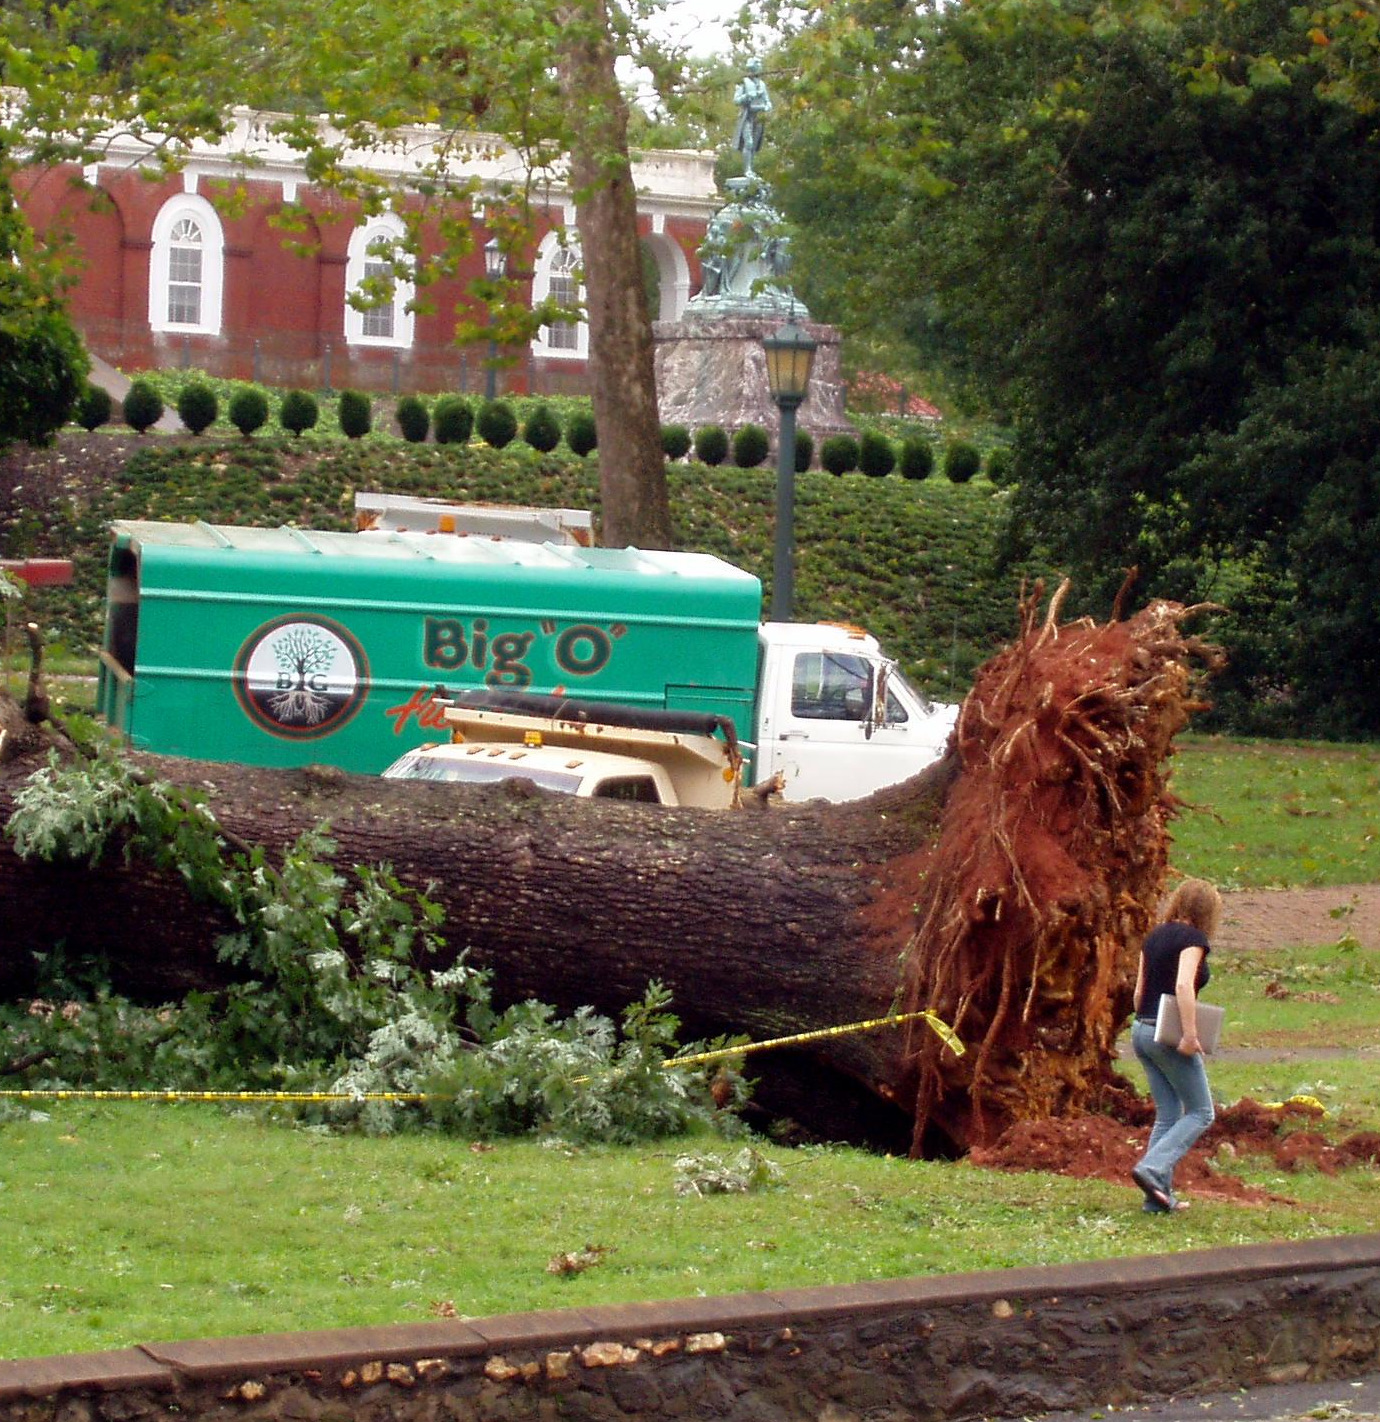
\includegraphics[width=2.4in]{images/edit/unbalanced-tree-edit-normalize-P1010045.jpg}
\vspace*{0.2cm}
%\scalebox{0.6}{\includegraphics{images/unbalanced-tree-normalize-P1010045.JPG}}
\end{minipage}
}
\caption{Unbalanced trees.}\label{fig:unbalanced}
\end{figure}

\begin{comment}
\begin{figure}[!bh]
{\centering
\begin{minipage}[t]{2.3in}\centering
\Tree[-1]{ \K{\snumber{1}} \B{dr} \\
          & \K{\snumber{5}} \B{dr} \\
          & & \K{\snumber{6}} \B{dr} \\
          & & & \K{\snumber{7}} \B{dr} \\
          & & & & \K{\snumber{12}} \B{dr} \\
          & & & & & \K{\snumber{17}}}
\end{minipage}
\begin{minipage}[t]{1.0in}
%\vspace*{0.3cm}
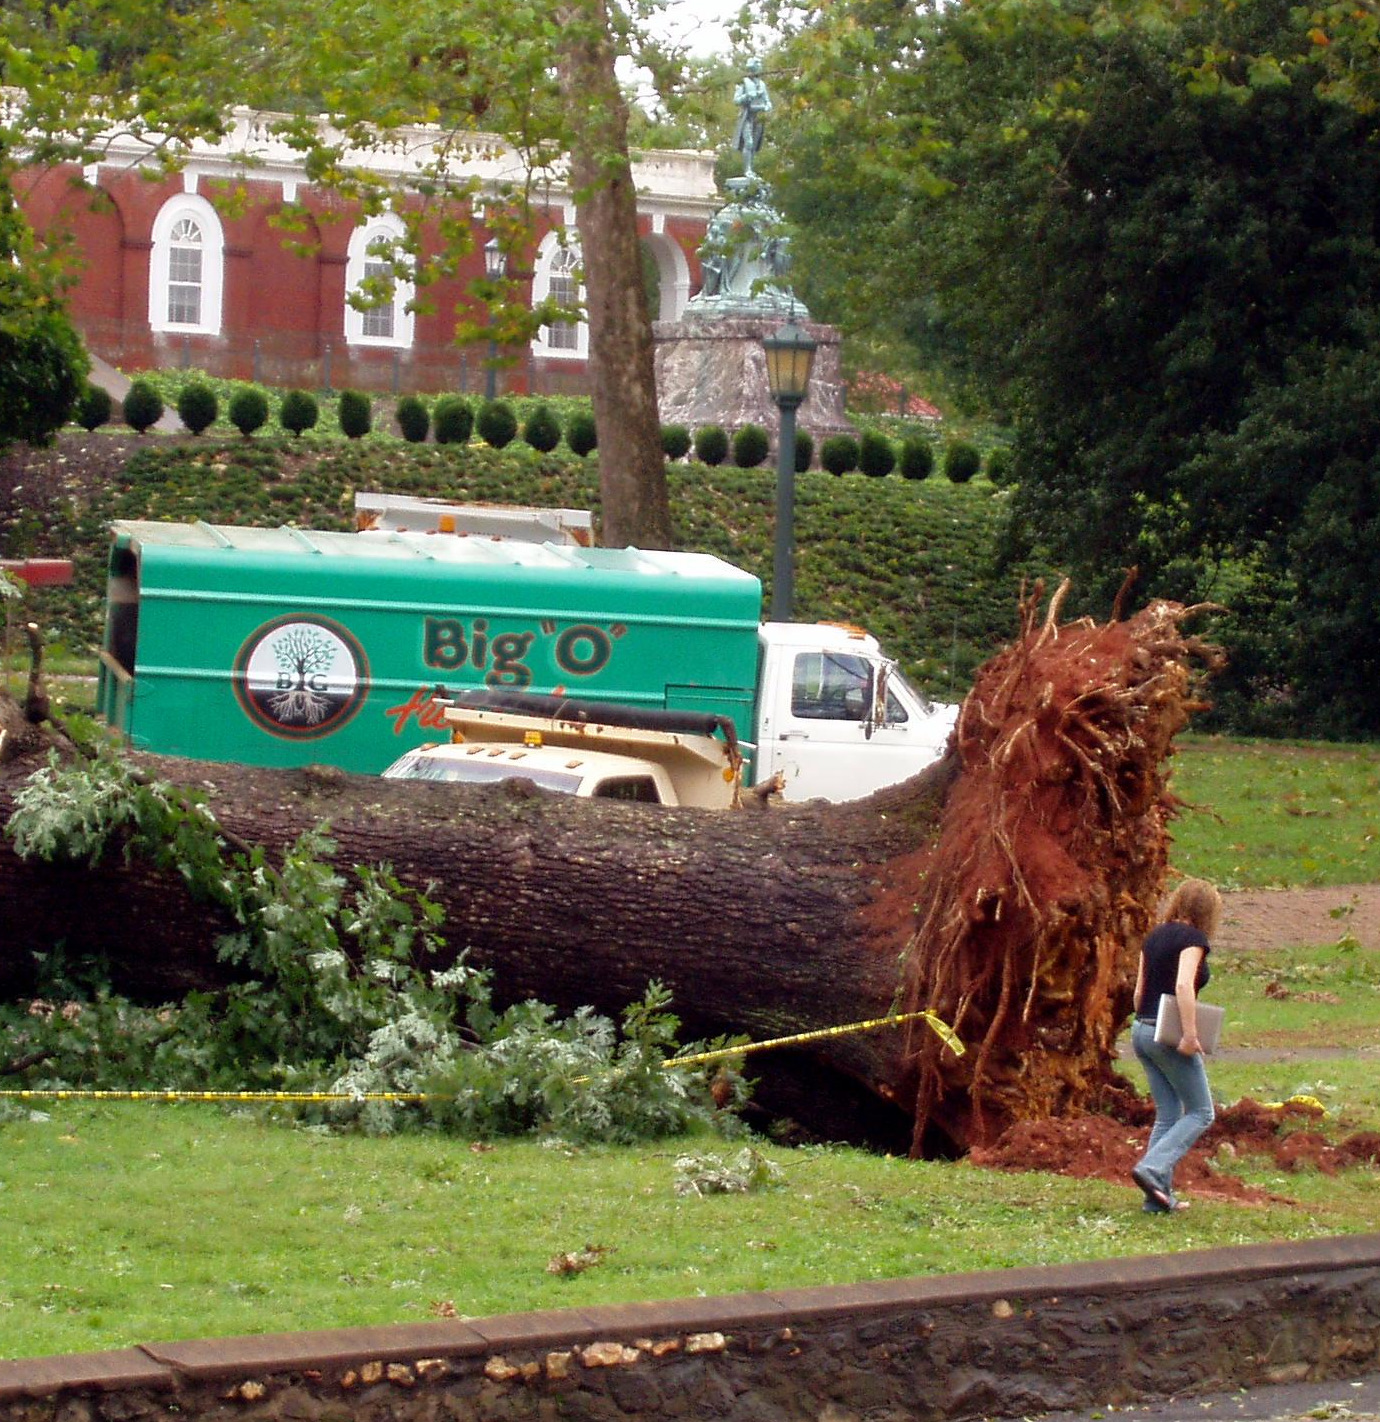
\includegraphics[width=0.95in]{images/edit/unbalanced-tree-edit-normalize-P1010045.jpg}
\end{minipage}
}
\caption{Unbalanced trees.}\label{fig:unbalanced}
\end{figure}
\end{comment}

In these pathological situations, the tree effectively becomes a list.  The number of recursive applications of \scheme|tree-insert-one| needed to insert a new element will not be in $\Theta(\log n)$, but rather will be in $\Theta(n)$.  Hence, the worst case running time for \scheme{list-sort-tree-insert} is in $\Theta(n^2)$ since the worst case time for \scheme|tree-insert-one| is in $\Theta(n)$ and there are $\Theta(n)$ applications of \scheme|tree-insert-one|.  The \scheme|list-sort-tree-insert| procedure has expected running time in $\Theta(n \log n)$ for randomly distributed inputs, but has worst case running time in $\Theta(n^2)$.

\beforeex
\begin{exercise}
Define a procedure \scheme|binary-tree-size| that takes as input a binary tree and outputs the number of elements in the tree.  Analyze the running time of your procedure.
\solution{\LATER{}}
\end{exercise}
\afterex

\beforeex
\begin{exercise}\goldstar 
Define a procedure \scheme|binary-tree-depth| that takes as input a binary tree and outputs the depth of the tree.  \cut{Recall that the depth of a binary tree is the length of the \emph{longest} path from the root to any node in the tree.}  The running time of your procedure should not grow faster than linearly with the number of nodes in the tree.
\solution{\LATER{}}
\end{exercise}
\afterex

\beforesplitex
\begin{exercise}\doublegoldstar 
Define a procedure \scheme|binary-tree-balance| that takes as input a sorted binary tree and the comparison function, and outputs a sorted binary tree containing the same elements as the input tree but in a well-balanced tree.  The depth of the output tree should be no higher than $\log_2 n + 1$ where $n$ is the number of elements in the input tree.
\solution{\LATER{}}
\end{exercise}
\aftersplitex 

\subsection{Quicksort} \label{sec:quicksort}

\sidequote{My first task was to implement %$\ldots$\cut{for the new Elliott 803 computer,} 
a library subroutine for a new fast method of internal sorting just invented by Shell$\ldots$\cut{ I greatly enjoyed the challenge of maximizing efficiency in the simple decimal-addressed machine code of those days.} My boss and tutor, Pat Shackleton, was very pleased with my completed program. I then said timidly that I thought I had invented a sorting method that would usually run faster than Shell sort, without taking much extra store. He bet me sixpence that I had not. Although my method was very difficult to explain, he finally agreed that I had won my bet.}{Sir Tony Hoare, \emph{The Emperor's Old Clothes}, 1980 Turing Award Lecture. (Shell sort is a $\Theta(n^2)$ sorting algorithm, somewhat similar to insertion sort.)} Although building and extracting elements from trees allows us to sort with expected time in $\Theta(n\log n)$, the constant time required to build all those trees and extract the elements from the final tree is high.  

In fact, we can use the same approach to sort without needing to build trees.  Instead, we keep the two sides of the tree as separate lists, and sort them recursively.  The key is to divide the list into halves by \emph{value}, instead of by \emph{position}.  The values in the first half of the list are all less than the values in the second half of the list, so the lists can be sorted separately.

The \scheme|list-quicksort| procedure uses \scheme|list-filter| (from Example~\ref{example:filter}) to divide the input list into sublists containing elements below and above the comparison element, and then recursively sorts those sublists:
\begin{schemedisplay}
(define (list-quicksort cf p)
  (if (null? p) null
      (list-append 
       (list-quicksort cf 
        (list-filter (lambda (el) (cf el (car p))) (cdr p)))
       (cons (car p)
             (list-quicksort cf 
              (list-filter (lambda (el) (not (cf el (car p)))) (cdr p)))))))
\end{schemedisplay}
This is the famous \emph{quicksort} algorithm that was invented by Sir C. A. R. (Tony) Hoare while he was an exchange student at Moscow State University in 1959.  
He was there to study probability theory, but also got a job working on a project to translate Russian into English.  The translation depended on looking up words in a dictionary.  Since the dictionary was stored on a magnetic tape which could be read in order faster than if it was necessary to jump around, the translation could be done more quickly if the words to translate were sorted alphabetically.  Hoare invented the quicksort algorithm for this purpose and it remains the most widely used sorting algorithm.  
%%! \sidepicture{0.36}{images/tonyhoare.jpg}{Sir Tony Hoare}{Photo by Gesp\"{u}r f\"{u}r Licht} %http://farm1.static.flickr.com/14/18059501_7474b38f94.jpg?v=0 % photo by: Gesp�r f�r Licht's
\cut{A few years later, he worked for Elliot Brothers, a small British computer manufacturer.  His first assignment there was to implement a sorting library procedure for a new machine they were developing. Quicksort proved to be faster than the best previously known sorting algorithms, and remains the most widely used sorting algorithm. }
%http://delivery.acm.org/10.1145/70000/63445/cb-p19-hoare.pdf?key1=63445&key2=5545355321&coll=&dl=GUIDE&CFID=15151515&CFTOKEN=6184618
%\LATER{Add story about quicksort}

As with \scheme|list-sort-tree-insert|, the expected running time for a randomly arranged list is in $\Theta(n\log n)$ and the worst case running time is in $\Theta(n^2)$.  In the expected cases, each recursive call halves the size of the input list (since if the list is randomly arranged we expect about half of the list elements are below the value of the first element), so there are approximately $\log n$ expected recursive calls.  

Each call involves an application of \scheme|list-filter|, which has running time in $\Theta(m)$ where $m$ is the length of the input list.  At each call depth, the total length of the inputs to all the calls to \scheme|list-filter| is $n$ since the original list is subdivided into $2^d$ sublists, which together include all of the elements in the original list.  Hence, the total running time is in $\Theta(n\log n)$ in the expected cases where the input list is randomly arranged.  As with \scheme|list-sort-tree-insert|, if the input list is not randomly rearranged it is possible that all elements end up in the same partition.  Hence, the worst case running time of \scheme|list-quicksort| is still in $\Theta(n^2)$. 

\sidequote{There are two ways of constructing a software design: one way is to make it so simple that there are {\em obviously} no deficiencies, and the other way is to make it so complicated that there are no {\em obvious} deficiencies.  The first method is far more difficult.  It demands the same skill, devotion, insight, and even inspiration as the discovery of the simple physical laws which underlie the complex phenomena of nature.}{Sir Tony Hoare, \emph{The Emperor's Old Clothes} (1980 Turing Award Lecture)}

\beforeex
\begin{exercise}
Estimate the time it would take to sort a list of one million elements using \scheme|list-quicksort|.
\solution{\LATER{}}
\end{exercise}
\afterex

\beforeex
\begin{exercise}
Both the \scheme|list-quicksort| and \scheme|list-sort-tree-insert| procedures have expected running times in $\Theta(n\log n)$.  Experimentally compare their actual running times.
\solution{\LATER{}}
\end{exercise}
\afterex

\beforeex
\begin{exercise}
What is the best case input for \scheme|list-quicksort|?  Analyze the asymptotic running time for \scheme|list-quicksort| on best case inputs.
\solution{\LATER{}}
\end{exercise}
\afterex

\beforeex
\begin{exercise} \goldstar 
Instead of using binary trees, we could use ternary trees.  A node in a ternary tree has two elements, a left element and a right element, where the left element must be before the right element according to the comparison function.  Each node has three subtrees: \scheme|left|, containing elements before the left element; \scheme|middle|, containing elements between the left and right elements; and \scheme|right|, containing elements after the right element.  Is it possible to sort faster using ternary trees?
\solution{\LATER{}}
\end{exercise}
\afterex

\index{general}{sorting|)}

%\LATER{Built-in sort procedure}
%\footnote{We follow the convention of the built-in \scheme|sort| procedure by making the input list the first parameter, and the sorting procedure the second parameter.  This is the opposite order from most of our other procedures, in which the procedure parameter is first.}

\section{Searching}\label{sec:searching}\index{general}{searching}

In a broad sense, nearly all problems can be thought of as search problems.  If we can define the space of possible solutions, we can search that space to find a correct solution.  For example, to solve the pegboard puzzle (Exploration~\ref{exploration:pegboard}) we enumerate all possible sequences of moves and search that space to find a winning sequence.\index{general}{pegboard puzzle}  For most interesting problems, however, the search space is far too large to search through all possible solutions.

This section explores a few specific types of search problems.  First, we consider the simple problem of finding an element in a list that satisfies some property.  Then, we consider searching for an item in sorted data.  Finally, we consider the more specific problem of efficiently searching for documents (such as web pages) that contain some target word.

\subsection{Unstructured Search}\label{sec:linearsearch}\index{general}{list-search}

Finding an item that satisfies an arbitrary property in unstructured data requires testing each element in turn until one that satisfies the property is found.  Since we have no more information about the property or data, there is no way to more quickly find a satisfying element.  

The \scheme|list-search| procedure takes as input a matching function and a list, and outputs the first element in the list that satisfies the matching function or \schemeresult|false| if there is no satisfying element:\footnote{If the input list contains \scheme|false| as an element, we do not know when the \scheme|list-search| result is \schemeresult|false| if it means the element is not in the list or the element whose value is \scheme|false| satisfies the property.  An alternative would be to produce an error if no satisfying element is found, but this is more awkward when \scheme|list-search| is used by other procedures.}
\begin{schemedisplay}
(define (list-search ef p)
  (if (null? p) false ; Not found
      (if (ef (car p)) (car p) (list-search ef (cdr p)))))
\end{schemedisplay}

For example,
\begin{code}
\scheme|(list-search (lambda (el) (= 12 el)) (intsto 10))| \evalsto \schemeresult|false|\\
\scheme|(list-search (lambda (el) (= 12 el)) (intsto 15))| \evalsto \schemeresult|12|\\
\scheme|(list-search (lambda (el) (> el 12)) (intsto 15))| \evalsto \schemeresult|13|
\end{code}

Assuming the matching function has constant running time, the worst case running time of \scheme|list-search| is linear in the size of the input list.  The worst case is when there is no satisfying element in the list.  If the input list has length $n$, there are $n$ recursive calls to \scheme|list-search|, each of which involves only constant time procedures.  

Without imposing more structure on the input and comparison function, there is no more efficient search procedure.  In the worst case, we always need to test every element in the input list before concluding that there is no element that satisfies the matching function.

\subsection{Binary Search}\label{sec:binarysearch}\index{general}{binary tree}\index{general}{binary search}

If the data to search is structured, it may be possible to find an element that satisfies some property without examining all elements.  Suppose the input data is a sorted binary tree, as introduced in Section~\ref{sec:binary-trees}.  Then, with a single comparison we can determine if the element we are searching for would be in the left or right subtree.  Instead of eliminating just one element with each application of the matching function as was the case with \scheme|list-search|, with a sorted binary tree a single application of the comparison function is enough to exclude approximately half the elements.

The \scheme|binary-tree-search| procedure takes a sorted binary tree and two procedures as its inputs.  The first procedure determines when a satisfying element has been found (we call this the \scheme|ef| procedure, suggesting equality).  The second procedure, \scheme|cf|, determines whether to search the left or right subtree.  Since \scheme|cf| is used to traverse the tree, the input tree must be sorted by \scheme|cf|.

\begin{schemedisplay}
(define (binary-tree-search ef cf tree) ; requires: tree is sorted by cf
  (if (null? tree) false
      (if (ef (tree-element tree)) (tree-element tree)
          (if (cf (tree-element tree))
              (binary-tree-search ef cf (tree-left tree))
              (binary-tree-search ef cf (tree-right tree))))))
\end{schemedisplay}

For example, we can search for a number in a sorted binary tree using \scheme|=| as the equality function and \scheme|<| as the comparison function:\cut{ (which must be the same as the comparison function used to build the tree).}
\begin{schemedisplay}
(define (binary-tree-number-search tree target)
 (binary-tree-search (lambda (el) (= target el))
                     (lambda (el) (< target el)) 
                     tree))
\end{schemedisplay}

To analyze the running time of \scheme|binary-tree-search|, we need to determine the number of recursive calls.  Like our analysis of \scheme|list-sort-tree|, we assume the input tree is well-balanced.  If not, all the elements could be in the right branch, for example, and \scheme|binary-tree-search| becomes like \scheme|list-search| in the pathological case.  

If the tree is well-balanced, each recursive call approximately halves the number of elements in the input tree since it passed in either the left or right subtree.  Hence, the number of calls needed to reach a \scheme|null| tree is in $\Theta(\log n)$ where $n$ is the number of elements in the input tree.  This is the depth of the tree: \scheme|binary-tree-search| traverses \emph{one} path from the root through the tree until either reaching an element that satisfies the \scheme|ef| function, or reaching a \scheme|null| node.  
%\sidepicturenocap{0.28}{images/yosemite-trees-IMG_0693.JPG}

Assuming the procedures passed as \scheme|ef| and \scheme|cf| have constant running time, the work for each call is constant except for the recursive call.  Hence, the total running time for \scheme|binary-tree-search| is in $\Theta(\log n)$ where $n$ is the number of elements in the input tree.  This is a huge improvement over linear searching: with linear search, doubling the number of elements in the input doubles the search time; with binary search, doubling the input size only increases the search time by a constant.  

\subsection{Indexed Search}\label{sec:indexed-search}\index{general}{indexed search}

The limitation of binary search is we can only use is when the input data is already sorted.  What if we want to search a collection of documents, such as finding all web pages that contain a given word?  
The web visible to search engines contains billions of web pages\cut{\footnote{Google's database reached 1 trillion unique web addresses in July 2008.}} most of which contain hundreds or thousands of words.  A linear search over such a vast corpus would be infeasible: supposing each word can be tested in 1 millisecond, the time to search 1 trillion words would be over 30 years!

Providing useful searches over large data sets like web documents requires finding a way to structure the data so it is not necessary to examine all documents to perform a search.  One way to do this is to build an index that provides a mapping from words to the documents that contain them.  Then, we can build the index once, store it in a sorted binary tree, and use it to perform all the searches.  Once the index is built, the work required to perform one search is just the time it takes to look up the target word in the index.  If the index is stored as a sorted binary tree, this is logarithmic in the number of distinct words.

\shortsection{Strings}\index{general}{String}  We use the built-in String datatype to represent documents and target words.  A String is similar to a List, but specialized for representing sequences of characters.  A convenient way to make a String it to just use double quotes around a sequence of characters.  For example, \scheme|"abcd"| evaluates to a String containing four characters.  

The String datatype provides procedures for matching, ordering, and converting between Strings and Lists of characters:
\begin{descriptionlist}
\item [\scheme|string=?|: String $\times$ String $\rightarrow$ Boolean] \forcenl Outputs \schemeresult|true| if the input Strings have exactly the same sequence of characters, otherwise \schemeresult|false|.
\item [\scheme|string<?|: String $\times$ String $\rightarrow$ Boolean] \forcenl Outputs \schemeresult|true| if the first input String is lexicographically before the second input String, otherwise \schemeresult|false|.  
\item [\scheme|string->list|: String $\rightarrow$ List] \forcenl Outputs a List containing the characters in the input String.
\item [\scheme|list->string|: List $\rightarrow$ String] \forcenl Outputs a String containing the characters in the input List.
\end{descriptionlist}
One advantage of using Strings instead of Lists of characters\cut{is the String representation of \verb|"abcd"| displays as a \schemeresult|"abcd"| which is easier to read than the List representation: \schemeresult|(#\a #\b #\c #\d)|.  Another advantage} is the built-in procedures for comparing Strings; we could write similar procedures for Lists of characters, but lexicographic ordering is somewhat tricky to get right, so it is better to use the built-in procedures.

\shortsection{Building the index} The entries in the index are Pairs of a word represented as a string, and a list of locations where that word appears.  Each location is a Pair consisting of a document identifier (for web documents, this is the Uniform Resource Locator (URL) that is the address of the web page represented as a string) and a Number identifying the position within the document where the word appears (we label positions as the number of characters in the document before this location).  

To build the index, we split each document into words and record the position of each word in the document.  The first step is to define a procedure that takes as input a string representing an entire document, and produces a list of \scheme|(word . position)| pairs containing one element for each word in the document.  We define a word as a sequence of alphabetic characters; non-alphabetic characters including spaces, numbers, and punctuation marks separate words and are not included in the index.  

The \scheme|text-to-word-positions| procedure takes a string as input and outputs a list of word-position pairs corresponding to each word in the input.  The inner procedure, \scheme|text-to-word-positions-iter|, takes three inputs: a list of the characters in the document, a list of the characters in the current word, and a number representing the position in the string where the current word starts; it outputs the list of \scheme|(word . position)| pairs.  The value passed in as \scheme|w| can be \scheme|null|, meaning there is no current word.  Otherwise, it is a list of the characters in the current word.  A word starts when the first alphabetic character is found, and continues until either the first non-alphabetic character or the end of the document.  We use the built-in \scheme|char-downcase| procedure to convert all letters to their lowercase form, so \keyword{KING}, \keyword{King}, and \keyword{king} all correspond to the same word.  

\begin{schemedisplay}
(define (text-to-word-positions s)
  (define (text-to-word-positions-iter p w pos)
    (if (null? p)
        (if (null? w) null (list (cons (list->string w) pos)))
        (if (not (char-alphabetic? (car p))) ; finished word
            (if (null? w) ; no current word
                (text-to-word-positions-iter (cdr p) null (+ pos 1))
                (cons (cons (list->string w) pos)
                      (text-to-word-positions-iter (cdr p) null 
                       (+ pos (list-length w) 1))))
            (text-to-word-positions-iter (cdr p) 
             (list-append w (list (char-downcase (car p)))) 
             pos))))
  (text-to-word-positions-iter (string->list s) null 0))
\end{schemedisplay}

The next step is to build an index from the list of word-position pairs.  To enable fast searching, we store the index in a binary tree sorted by the target word.  The \scheme|insert-into-index| procedure takes as input an index and a word-position pair and outputs an index consisting of the input index with the input word-position pair added.  

The index is represented as a sorted binary tree where each element is a pair of a word and a list of the positions where that word appears.  Each word should appear in the tree only once, so if the word-position pair to be added corresponds to a word that is already in the index, the position is added to the corresponding list of positions.  Otherwise, a new entry is added to the index for the word with a list of positions containing the position as its only element.

\begin{schemedisplay}
(define (insert-into-index index wp)
  (if (null? index)
      (make-tree null (cons (car wp) (list (cdr wp))) null)
      (if (string=? (car wp) (car (tree-element index)))
          (make-tree (tree-left index)
                     (cons (car (tree-element index))
                           (list-append (cdr (tree-element index)) 
                                        (list (cdr wp))))
                     (tree-right index))
          (if (string<? (car wp) (car (tree-element index)))
              (make-tree (insert-into-index (tree-left index) wp)
                         (tree-element index)
                         (tree-right index))
              (make-tree (tree-left index)
                         (tree-element index)
                         (insert-into-index (tree-right index) wp))))))
\end{schemedisplay}  

To insert all the \scheme|(word . position)| pairs in a list into the index, we use \scheme|insert-into-index| to add each pair, passing the resulting index into the next recursive call:
\begin{schemedisplay}  
(define (insert-all-wps index wps)
  (if (null? wps) index
      (insert-all-wps (insert-into-index index (car wps)) (cdr wps))))
\end{schemedisplay}

To add all the words in a document to the index we use \scheme|text-to-word-positions| to obtain the list of word-position pairs.  Since we want to include the document identity in the positions, we use \scheme|list-map| to add the \scheme|url| (a string that identifies the document location) to the position of each word.  Then, we use \scheme|insert-all-wps| to add all the word-position pairs in this document to the index.  The \scheme|index-document| procedure takes a document identifier and its text as a string, and produces an index of all words in the document.
\begin{schemedisplay}
(define (index-document url text)
  (insert-all-wps
   null
   (list-map (lambda (wp) (cons (car wp) (cons url (cdr wp))))
             (text-to-word-positions text))))
\end{schemedisplay}

We leave analyzing the running time of \scheme|index-document| as an exercise.  The important point, though, is that it only has to be done once for a given set of documents.  Once the index is built, we can use it to answer any number of search queries without needing to reconstruct the index.  %Large search engine companies dedicate large numbers of machines to maintaining the index as new web pages are found.

\shortsection{Merging indexes} Our goal is to produce an index for a set of documents, not just a single document.  So, we need a way to take two indexes produced by \scheme|index-document| and combine them into a single index.  We use this repeatedly to create an index of any number of documents.  To merge two indexes, we combine their word occurrences.  If a word occurs in both documents, the word should appear in the merged index with a position list that includes all the positions in both indexes.  If the word occurs in only one of the documents, that word and its position list should be included in the merged index.  

\begin{schemedisplay}
(define (merge-indexes d1 d2)
  (define (merge-elements p1 p2)
    (if (null? p1) p2
        (if (null? p2) p1
            (if (string=? (car (car p1)) (car (car p2)))
                (cons (cons (car (car p1))
                            (list-append (cdr (car p1)) (cdr (car p2))))
                      (merge-elements (cdr p1) (cdr p2)))
                (if (string<? (car (car p1)) (car (car p2)))
                    (cons (car p1) (merge-elements (cdr p1) p2))
                    (cons (car p2) (merge-elements p1 (cdr p2))))))))
  (list-to-sorted-tree
   (lambda (e1 e2) (string<? (car e1) (car e2)))
   (merge-elements (tree-extract-elements d1) 
                   (tree-extract-elements d2))))
\end{schemedisplay}
To merge the indexes, we first use \scheme|tree-extract-elements| to convert the tree representations to lists.  The inner \scheme|merge-elements| procedure takes the two lists of word-position pairs and outputs a single list.  

Since the lists are sorted by the target word, we can perform the merge efficiently.  If the first words in both lists are the same, we produce a word-position pair that appends the position lists for the two entries.  If they are different, we use \scheme|string<?| to determine which of the words belongs first, and include that element in the merged list.  This way, the two lists are kept synchronized, so there is no need to search the lists to see if the same word appears in both lists.  

\shortsection{Obtaining documents} To build a useful index for searching, we need some documents to index.  The web provides a useful collection of freely available documents.  To read documents from the web, we use library procedures provided by DrRacket.  \index{general}{web}\index{general}{URL}

This expression loads the libraries for managing URLs and getting files from the network: \scheme|(require (lib "url.ss" "net"))|.  One procedure this library defines is \scheme|string->url|, which takes a string as input and produces a representation of that string as a URL. A Uniform Resource Locator (URL) is a standard way to identify a document on the network.  The address bar in most web browsers displays the URL of the current web page.  

The full grammar for URLs is quite complex (see Exercise~\ref{exercise:domains}), but we will use simple web page addresses of the form:\footnote{We use \nonterminal{Name} to represent sequences of characters in the domain and path names, although the actual rules for valid names for each of these are different.}
\begin{bnfgrammarm}{SubDomains}
\bnfrule{URL}{\terminal{http://} \nonterminal{Domain} \nonterminal{OptPath}}
\bnfrule{Domain}{\nonterminal{Name} \nonterminal{SubDomains}}
\bnfrule{SubDomains}{\terminal{.} \nonterminal{Domain}}
\bnfrule{SubDomains}{$\epsilon$}
\bnfrule{OptPath}{Path}
\bnfrule{OptPath}{$\epsilon$}
\bnfrule{Path}{\terminal{/} \nonterminal{Name} \nonterminal{OptPath}}
\end{bnfgrammarm}
An example of a URL is \url{http://www.whitehouse.gov/index.html}.  The \url{http} indicates the HyperText Transfer Protocol, which prescribes how the web client (browser) and server communicate with each other.  The domain name is \url{www.whitehouse.gov}, and the path name is \url{/index.html} (which is the default page for most web servers).

The library also defines the \scheme|get-pure-port| procedure that takes as input a URL and produces a port for reading the document at that location.  The \scheme|read-char| procedure takes as input a port, and outputs the first character in that port.  It also has a side effect: it advances the port to the next character.  We can use \scheme|read-char| repeatedly to read each character in the web page of the port.  When the end of the file is reached, the next application of \scheme|read-char| outputs a special marker representing the end of the file.  The procedure \scheme|eof-object?| evaluates to \schemeresult|true| when applied to this marker, and \schemeresult|false| for all other inputs.

The \scheme|read-all-chars| procedure takes a port as its input, and produces a list containing all the characters in the document associated with the port:
\begin{schemedisplay}
(define (read-all-chars port)
  (let ((c (read-char port)))
    (if (eof-object? c) null 
        (cons c (read-all-chars port)))))
\end{schemedisplay}

Using these procedures, we define \scheme|web-get|, a procedure that takes as input a string that represents the URL of some web page, and outputs a string representing the contents of that page.\index{general}{web-get}
\begin{schemedisplay}         
(define (web-get url)
  (list->string (read-all-chars (get-pure-port (string->url url)))))
\end{schemedisplay}

To make it easy to build an index of a set of web pages, we define the \scheme|index-pages| procedure that takes as input a list of web pages and outputs an index of the words in those pages.  It recurses through the list of pages, indexing each document, and merging that index with the result of indexing the rest of the pages in the list.

\begin{schemedisplay}
(define (index-pages p)
  (if (null? p) null
      (merge-indexes (index-document (car p) (web-get (car p))) 
                     (index-pages (cdr p)))))
\end{schemedisplay}

We can use this to create an index of any set of web pages.  For example, here we use Jeremy Hylton's collection of the complete works of William Shakespeare (\url{http://shakespeare.mit.edu}) to define \scheme|shakespeare-index| as an index of the words used in all of Shakespeare's plays.

\begin{schemedisplay}
(define shakespeare-index 
  (index-pages
   (list-map
    (lambda (play) 
     (string-append "http://shakespeare.mit.edu/" play "/full.html"))
     ;; List of plays following the site's naming conventions.
    (list "allswell" "asyoulikeit" "comedy_errors" "cymbeline" "lll" 
     "measure" "merry_wives" "merchant" "midsummer" "much_ado" 
     "pericles" "taming_shrew" "tempest" "troilus_cressida" "twelfth_night" 
     "two_gentlemen" "winters_tale" "1henryiv" "2henryiv" "henryv" 
     "1henryvi" "2henryvi" "3henryvi" "henryviii" "john" "richardii" 
     "richardiii" "cleopatra" "coriolanus" "hamlet" "julius_caesar" "lear" 
     "macbeth" "othello" "romeo_juliet" "timon" "titus"))))
\end{schemedisplay}
Building the index takes about two and a half hours on my laptop.  It contains 22949 distinct words and over 1.6 million word occurrences.  Much of the time spent building the index is in constructing new lists and trees for every change, which can be avoided by using the mutable data types we cover in the next chapter.  The key idea, though, is that the index only needs to be built once.  Once the documents have been indexed, we can use the index to quickly perform any search.

\shortsection{Searching}  Using an index, searching for pages that use a given word is easy and efficient.  Since the index is a sorted binary tree, we use \scheme|binary-tree-search| to search for a word in the index:
\begin{schemedisplay}
(define (search-in-index index word)
  (binary-tree-search
   (lambda (el) (string=? word (car el))) ; first element of (word . position)
   (lambda (el) (string<? word (car el)))
   index))
\end{schemedisplay}

As analyzed in the previous section, the expected running time of \scheme|binary-tree-search| is in $\Theta(\log n)$ where $n$ is the number of nodes in the input tree.\footnote{Because of the way \scheme|merge-indexes| is defined, we do not actually get this expected running time.  See Exercise~\ref{exercise:merge}.} The body of \scheme|search-in-index| applies \scheme|binary-tree-search| to the index.  The number of nodes in the index is the number of distinct words in the indexed documents.  So, the running time of \scheme|search-in-index| scales logarithmically with the number of distinct words in the indexed documents.  Note that the number and size of the documents does not matter!  This is why a search engine such as Google can respond to a query quickly even though its index contains many billions of documents.  

One issue we should be concerned with is the running time of the procedures passed into \scheme|binary-tree-search|.  Our analysis of \scheme|binary-tree-search| assumes the equality and comparison functions are constant time procedures.  Here, the procedures as \scheme|string=?| and \scheme|string<?|, which both have worst case running times that are linear in the length of the input string.  As used here, one of the inputs is the target word.  So, the amount of work for each \scheme|binary-tree-search| recursive call is in $\Theta(w)$ where $w$ is the length of \scheme|word|.  Thus, the overall running time of \scheme|search-in-index| is in $\Theta(w \log d)$ where $w$ is the length of \scheme|word| and $d$ is the number of words in the \scheme|index|.  If we assume all words are of some maximum length, though, the $w$ term disappears as a constant factor (that is, we are assuming $w < C$ for some constant $C$.  Thus, the overall running time is in $\Theta(\log d)$.

Here are some examples: % uses of \scheme|search-in-index| using our index of Shakespeare's plays:
\begin{code}\LATER{FIXSPACING}
\scheme|> (search-in-index shakespeare-index "mathematics")|\\
\sidequote{The mathematics and the meta\-physics,
Fall to them as you find your stomach serves you;
No profit grows where is no pleasure ta'en:
In brief, sir, study what you most affect.}{William~Shakespeare, \emph{The~Taming of the~Shrew}}
\schemeresult|("mathematics"|\\
\schemeresult|\squad ("http://shakespeare.mit.edu/taming_shrew/full.html" . 26917)|\\
\schemeresult|\squad ("http://shakespeare.mit.edu/taming_shrew/full.html" . 75069)|\\
\schemeresult|\squad ("http://shakespeare.mit.edu/taming_shrew/full.html" . 77341))|\\
\scheme|> (search-in-index shakespeare-index "procedure")|\\
\schemeresult|false|\\
%\scheme|> (search-in-index shakespeare-index "abstraction")|\\
%\schemeresult|false|\\
\end{code}

Our \scheme|search-in-index| and \scheme|index-pages| procedures form the beginnings of a search engine service.  A useful web search engine needs at least two more capabilities: a way to automate the process of finding documents to index, and a way to rank the documents that contain the target word by the likelihood they are useful.  The exploration at the end of this section addresses these capabilities.

\shortsection{Histogram} We can also use our index to analyze Shakespeare's writing.  The \scheme|index-histogram| procedure produces a list of the words in an index sorted by how frequently they appear:  
\begin{schemedisplay}
(define (index-histogram index)
  (list-quicksort 
   (lambda (e1 e2) (> (cdr e1) (cdr e2)))
   (list-map (lambda (el) (cons (car el) (length (cdr el))))
             (tree-extract-elements index))))
\end{schemedisplay}
The expression,
\begin{schemedisplay}
(list-filter (lambda (entry) (> string-length (car entry) 5)) 
             (index-histogram shakespeare-index))
\end{schemedisplay}             
evaluates to a list of Shakespeare's favorite 6-letter and longer words along with the number of times they appear in the corpus (the first two entries are from their use in the page formatting):
\begin{schemedisplay}
(("blockquote" . 63345) ("speech" . 31099) 
 ("should" . 1557) ("father" . 1086) ("exeunt" . 1061) 
 ("master" . 861) ("before" . 826) ("mistress" . 787)
 \ldots ("brother" . 623)
 \ldots ("daughter" . 452)
 \ldots ("mother" . 418)
 \ldots ("mustardseed" . 13)
 \ldots ("excrement" . 5)
 \ldots ("zwaggered" . 1))
\end{schemedisplay}
%The first two are words from the web page formatting markup, not from Shakespeare's writing.  The rest of the word frequencies provide a glimpse into Shakespeare's world.

\beforeex
\begin{exercise}
Define a procedure for finding the longest word in a document.  Analyze the running time of your procedure.
\solution{\LATER{}}
\end{exercise}
\afterex

\beforeex
\begin{exercise}
Produce a list of the words in Shakespeare's plays sorted by their length.
\solution{\LATER{}}
\end{exercise}
\afterex

\beforesplitex
\begin{exercise}\goldstar 
Analyze the running time required to build the index.
\begin{subexerciselist}
\item Analyze the running time of the \scheme|text-to-word-positions| procedure.  Use $n$ to represent the number of characters in the input string, and $w$ to represent the number of distinct words.  Be careful to clearly state all assumptions on which your analysis relies.
\solution{\LATER{}}
\item Analyze the running time of the \scheme|insert-into-index| procedure. 
\solution{\LATER{}}
\item Analyze the running time of the \scheme|index-document| procedure.  
\solution{\LATER{}}
\item Analyze the running time of the \scheme|merge-indexes| procedure.
\solution{\LATER{}}
\item Analyze the overall running time of the \scheme|index-pages| procedure.  Your result should describe how the running time is impacted by the number of documents to index, the size of each document, and the number of distinct words.
\solution{\LATER{}}
\end{subexerciselist}
\end{exercise}
\aftersplitex

\beforesplitex
\begin{exercise}\label{exercise:merge}\goldstar 
The \scheme|search-in-index| procedure does not actually have the expected running time in $\Theta(\log w)$ (where $w$ is the number of distinct words in the index) for the Shakespeare index because of the way it is built using \scheme|merge-indexes|.  The problem has to do with the running time of the binary tree on pathological inputs.  Explain why the input to \scheme|list-to-sorted-tree| in the \scheme|merge-indexes| procedure leads to a binary tree where the running time for searching is in $\Theta(w)$.  Modify the \scheme|merge-indexes| definition to avoid this problem and ensure that searches on the resulting index run in $\Theta(\log w)$.
\solution{\LATER{}}
\end{exercise}
\aftersplitex

\beforesplitex
\begin{exercise}\doublegoldstar 
The site \url{http://www.speechwars.com} provides an interesting way to view political speeches by looking at how the frequency of the use of different words changes over time.  \cut{For example, we can see that ``computer'' was first used in a state of the union speech by Jimmy Carter in 1981, and used five times by Bill Clinton, but not (yet) by any other president.} Use the \scheme|index-histogram| procedure to build a historical histogram program that takes as input a list of indexes ordered by time, and a target word, and output a list showing the number of occurrences of the target word in each of the indexes.  You could use your program to analyze how Shakespeare's word use is different in tragedies and comedies \cut{, how language on the web has changed over time (see \url{http://www.archive.org} for a way to obtain snapshots of web pages at particular times in the past),}or to compare Shakespeare's vocabulary to Jefferson's.
\solution{\LATER{}}
\end{exercise}
\aftersplitex

\clearpage %!!
\splitexplore{Searching the Web}{

In addition to fast indexed search, web search engines have to solve two problems: (1) find documents to index, and (2) identify the most important documents that contain a particular search term.

For our Shakespeare index example, we manually found a list of interesting documents to index.  This approach does not scale well to indexing the World Wide Web where there are trillions of documents and new ones are created all the time.  For this, we need a \definition{web crawler}.  

A web crawler finds documents on the web.  Typical web crawlers start with a set of seed URLs, and then find more documents to index by following the links on those pages.  This proceeds recursively: the links on each newly discovered page are added to the set of URLs for the crawler to index.  To develop a web crawler, we need a way to extract the links on a given web page, and to manage the set of pages to index.
\sidequote{The rank assigned to a document is calculated from the ranks of documents citing it. In addition, the rank of a document is calculated from a constant representing the probability that a browser through the database will randomly jump to the document. The method is particularly useful in enhancing the performance of search engine results for hypermedia databases, such as the world wide web, whose documents have a large variation in quality.}
{United States Patent \#6,285,999, September 2001.  (Inventor: Lawrence Page, Assignee: Stanford University)}

\begin{subexerciselist}
\item \goldstar Define a procedure \scheme|extract-links| that takes as input a string representing the text of a web page and outputs a list of all the pages linked to from this page.  Linked pages can be found by searching for anchor tags on the web page.  An anchor tag has the form:\footnote{Not all links match this structure exactly, so this may miss some of the links on a page.} $<${\sffamily a href=}\url{target}$>$.  (The \scheme|text-to-word-positions| procedure may be a helpful starting point for defining \scheme|extract-links|.)

\item \greenstar Define a procedure \scheme|crawl-page| that takes as input an index and a string representing a URL.  As output, it produces a pair consisting of an index (that is the result of adding all words from the page at the input URL to the input index) and a list of URLs representing all pages linked to by the crawled page.

\item \doublegoldstar Define a procedure \scheme|crawl-web| that takes as input a list of seed URLs and a Number indicating the maximum depth of the crawl.  It should output an index of all the words on the web pages at the locations given by the seed URLs and any page that can be reached from these seed URLs by following no more than the maximum depth number of links.
\suspend{subexerciselist}
For a web search engine to be useful, we don't want to just get a list of all the pages that contain some target word, we want the list to be sorted according to which of those pages are most likely to be interesting.  Selecting the best pages for a given query is a challenging and important problem, and the ability to do this well is one of the main things that distinguishes web search engines.  Many factors are used to rank pages including an analysis of the text on the page itself, whether the target word is part of a title, and how recently the page was updated.

The best ways of ranking pages also consider the pages that link to the ranked page.  If many pages link to a given page, it is more likely that the given page is useful.  This property can also be defined recursively: a page is highly ranked if there are many highly-ranked pages that link to it. 

The ranking system used by Google is based on this formula:
\begin{displaymath}
R(u) = \sum_{v \in L_u} \frac{R(v)}{L(v)}
\end{displaymath}
where $L_u$ is the set of web pages that contain links to the target page $u$ and $L(v)$ is the number of links on the page $v$ (thus, the value of a link from a page containing many links is less than the value of a link from a page containing only a few links).  The value $R(u)$ gives a measure of the ranking of the page identified by $u$, where higher values indicate more valuable pages.

The problem with this formula is that is is circular: there is no base case, and no way to order the web pages to compute the correct rank of each page in turn, since the rank of each page depends on the rank of the pages that link to it.  

One way to approximate equations like this one is to use \definition{relaxation}.  Relaxation obtains an approximate solution to some systems of equations by repeatedly evaluating the equations.  To estimate the page ranks for a set of web pages, we initially assume every page has rank 1 and evaluate $R(u)$ for all the pages (using the value of 1 as the rank for every other page).  Then, re-evaluate the $R(u)$ values using the resulting ranks.  A relaxation keeps repeating until the values change by less than some threshold amount, but there is no guarantee how quickly this will happen.  For the page ranking evaluation, it may be enough to decide on some fixed number of iterations.

\resume{subexerciselist}
\item \doublegoldstar Define a procedure, \scheme|web-link-graph|, that takes as input a set of URLs and produces as output a graph of the linking structure of those documents.  The linking structure can be represented as a List where each element of the List is a pair of a URL and a list of all the URLs that include a link to that URL.  The \scheme|extract-links| procedure from the previous exploration will be useful for determining the link targets of a given URL.

\item \goldstar Define a procedure that takes as input the output of \scheme|web-link-graph| and outputs a preliminary ranking of each page that measures the number of other pages that link to that page.  

\item \doublegoldstar Refine your page ranking procedure to weight links from highly-ranked pages more heavily in a page's rank by using a  algorithm.  

\item \quadgoldstar Come up with a cool name, set up your search engine as a web service, and attract more than 0.001\% of all web searches to your site.
\end{subexerciselist}
}

\section{Summary}

The focus of Part II has been on predicting properties of procedures, in particular how their running time scales with the size of their input.  This involved many encounters with the three powerful ideas introduced in Section~\ref{sec:roadmap}: recursive definitions, universality, and abstraction.  The simple Turing Machine model is a useful abstraction for modeling nearly all conceivable computing machines, and the few simple operations it defines are enough for a universal computer.  Actual machines use the digital abstraction to allow a continuous range of voltages to represent just two values.  The asymptotic operators used to describe running times are also a kind of abstraction---they allow us to represent the set of infinitely many different functions with a compact notation.  

In Part III, we will see many more recursive definitions, and extend the notion of recursive definitions to the language interpreter itself.  We change the language evaluation rules themselves, and see how different evaluation rules enable different ways of expressing computations.   

%In Part IV, we consider a deeper proble,: what is the running time of the fastest possible algorithm that solves a given problem.  Exploring this will allow us to understand what problems can %realistically be solved by computers, and what problems it is infeasible to solve with even much more powerful computers than we have today.


\cut{
As inventor of Quicksort, Sir Tony gets the last word:
\begin{quote}
{\em I quickly learned that the characteristic of a good course lasting one term is that after the first half of the course, the students just can't see what it is about at all, but at the end of the course they can't see what they found difficult anymore. So you have to choose a fixed time frame, and if you don't have that initial confusion and doubt you're probably not teaching things that are stretching your students enough.}
\flushright Tony Hoare, Charles~Babbage~Institute~Interview, July~2002
\end{quote}

We've covered a lot of material!  Don't despair if it doesn't all make sense yet.  The same concepts will recur frequently in the remainder of this book, and it takes lots of practice and many years to fully understand the implications of recursive definitions, higher order procedures, and abstraction.
}

%\end{comment}

\end{schemeregion}

\LATER{
\subsection{Problem Solving and the Growth of Computing Power}

In Chapter~\ref{ch:intro} (especially Section~\ref{sec:growthofcomputing}), we considered how computing power grows as technology improves over time and measured computing power according to the amount of memory available for a computation.  Now we can return to the question of computing power with the additional insight provided by the Chapters~\ref{ch:machines}--\ref{ch:cost}.  Since we can now reason about how the time it takes to evaluate a given procedure scales with the size of its input, we can make predictions about how the size of problem that can be solved scales over time.

\subsection{Where to Go From Here}


\subsection{Conclusion}
}
